\documentclass[11pt,a4paper]{article}

% ---------- Font & ngôn ngữ ----------
\usepackage{fontspec}
\usepackage{polyglossia}
\setmainlanguage{vietnamese}
% \setmainfont{Latin Modern Roman}

% ---------- Bố cục & định dạng ----------
\usepackage{geometry}
\geometry{a4paper, margin=2.5cm}
\usepackage{booktabs}
\usepackage{graphicx}
\usepackage{float}
\usepackage{enumitem}
\usepackage{listings}

\lstset{
    basicstyle=\small\ttfamily,
    frame=single,
    breaklines=true,
    showstringspaces=false
}

\setlength{\parskip}{0.4em}
\setlength{\parindent}{0pt}

\title{\textbf{BÁO CÁO MÔ PHỎNG GIAO THÔNG}\\[3pt]
\large So sánh ba phương pháp điều khiển đèn tín hiệu: \\
Cố định (Fixed-Time) -- Áp lực (MaxPressure) -- Trí tuệ nhân tạo (Q-Learning)}
\author{}
\date{}

\begin{document}

\maketitle

\section{Bối cảnh mô phỏng}

\subsection{Cấu trúc ngã tư và lưu lượng xe}
\begin{itemize}[leftmargin=*]
    \item Mỗi hướng có 6 làn xe.
    \item Có hai loại xe: ô tô (chiếm 40\% lượng xe) và xe máy (chiếm 60\%). Ô tô di chuyển nhanh hơn và chiếm nhiều diện tích hơn xe máy.
    \item Lưu lượng xe không đồng đều giữa hai trục: trục Bắc--Nam rất đông (trung bình 1,5 giây có một xe xuất hiện), trong khi trục Đông--Tây vắng hơn (trung bình 4,5 giây có một xe xuất hiện).
\end{itemize}

\subsection{Mô hình di chuyển an toàn}
\begin{itemize}[leftmargin=*]
    \item Các xe giữ khoảng cách an toàn với xe phía trước theo mô hình xe theo đuôi IDM: nếu xe phía trước đi chậm hoặc dừng lại, xe sau tự động giảm tốc để không va chạm.
    \item Xe đã đi vào khu vực giữa ngã tư thì cho phép đè lên nhau.
\end{itemize}

\section{Ba phương pháp điều khiển đèn tín hiệu}

\subsection{Phương pháp 1: Điều khiển thời gian cố định (Fixed-Time)}
\textbf{Cách hoạt động:} Đèn tín hiệu đổi màu theo một khoảng thời gian được lập trình sẵn, không phụ thuộc vào lượng xe thực tế trên đường.
\begin{itemize}[leftmargin=*]
    \item \textbf{Cài đặt:} 30 giây xanh cho trục Bắc--Nam $\rightarrow$ 3 giây vàng $\rightarrow$ 30 giây xanh cho trục Đông--Tây $\rightarrow$ 3 giây vàng. Chu kỳ lặp lại mỗi 66 giây.
\end{itemize}

\begin{lstlisting}[language=Java]
// Moi chu ky lap lai theo trinh tu co dinh
if (time_in_cycle < 30) {
    turnGreen(NorthSouth); // 30s xanh
} else if (time_in_cycle < 33) {
    turnYellow(NorthSouth); // 3s vang
} else if (time_in_cycle < 63) {
    turnGreen(EastWest); // 30s xanh
} else {
    turnYellow(EastWest); // 3s vang
}
\end{lstlisting}

\subsection{Phương pháp 2: Điều phối theo Max-Pressure}
\textbf{Cách hoạt động:} Lượng xe đang chờ trước đèn đỏ được coi là một loại "áp lực". Hướng nào có nhiều xe chờ hơn sẽ được ưu tiên bật đèn xanh.
\begin{itemize}[leftmargin=*]
    \item \textbf{Cơ chế tính toán:} Hệ thống liên tục đếm số xe đang tiến vào ngã tư và số xe đã thoát ra. Cứ mỗi 5 giây, nếu hướng đang chờ đèn đỏ có số xe nhiều hơn hướng đang được đi khoảng 2 xe trở lên, hệ thống sẽ chuyển pha đèn.
\end{itemize}

\begin{lstlisting}[language=Java]
// Tinh ap luc moi huong = (Xe dang den) - (Xe da qua)
pressure_NS = count_incoming(NS) - count_outgoing(NS);
pressure_EW = count_incoming(EW) - count_outgoing(EW);

// Doi den neu huong dang cho co ap luc lon hon huong dang di
if (current_green == NS && pressure_EW > pressure_NS + threshold) {
    switchTo(EW);
} else if (current_green == EW && pressure_NS > pressure_EW + threshold) {
    switchTo(NS);
}
\end{lstlisting}

\subsection{Phương pháp 3: Trí tuệ nhân tạo tự học (Q-Learning)}
\textbf{Cách hoạt động:} Hệ thống đóng vai trò một bộ điều khiển (AI Agent) tự quan sát tình hình ngã tư và rút kinh nghiệm sau mỗi lần điều khiển, theo nguyên lý học tăng cường (Reinforcement Learning).
\begin{itemize}[leftmargin=*]
    \item \textbf{Trạng thái (State):} AI quan sát pha đèn hiện tại và mức độ xe đang chờ ở mỗi hướng (ít, vừa, hoặc đông).
    \item \textbf{Hành động (Action):} Cứ mỗi 5 giây, AI quyết định giữ nguyên đèn xanh hoặc chuyển sang đèn đỏ.
    \item \textbf{Thưởng / phạt (Reward):} Nếu quyết định giúp ngã tư thông thoáng, AI nhận điểm thưởng; nếu khiến xe dồn ứ, AI nhận điểm phạt.
    \item \textbf{Kết quả:} Sau nhiều lần thử và điều chỉnh, hệ thống tự tìm ra cách chuyển đèn phù hợp với ngã tư này mà không cần con người lập trình thời gian cố định trước.
\end{itemize}

\begin{lstlisting}[language=Java]
// 1. Nhan dien trang thai hien tai (State)
state = getCurrentPhase() + "_" + getQueueLevel(NS) + "_" + getQueueLevel(EW);

// 2. Tra bang Q-Table de chon hanh dong tot nhat (Giu nguyen / Doi den)
action = chooseBestAction(state, Q_Table);
execute(action);

// 3. Quan sat ket qua va nhan phan thuong (Reward)
reward = - getTotalWaitingVehicles();
next_state = observeNewState();

// 4. Cap nhat kinh nghiem vao bang Q-Table (Phuong trinh Bellman)
Q_Table[state][action] = (1 - alpha) * Q_Table[state][action]
                         + alpha * (reward + gamma * max(Q_Table[next_state]));
\end{lstlisting}

\section{Kết quả mô phỏng}

Kết quả đo được của ba phương pháp được tổng hợp trong Bảng~\ref{tab:ketqua}.

\begin{table}[H]
\centering
\small
\caption{Bảng tổng hợp kết quả mô phỏng}
\label{tab:ketqua}
\begin{tabular}{lcccl}
\toprule
\textbf{Tiêu chí} & \textbf{Fixed-Time} & \textbf{MaxPressure} & \textbf{Q-Learning} & \textbf{Ghi chú} \\
\midrule
Tổng xe qua ngã tư & 112 xe & 105 xe & \textbf{109 xe} & Khá tương đương nhau \\
Thời gian chờ trung bình & 5,53 giây & 9,28 giây & \textbf{2,89 giây} & Giảm gần một nửa \\
Hàng đợi trung bình & 6,74 xe & 9,12 xe & \textbf{3,55 xe} & Hàng đợi ngắn nhất \\
Vận tốc trung bình & 16,85 km/h & 15,81 km/h & \textbf{19,09 km/h} & Xe di chuyển nhanh hơn \\
Thời gian mỗi chuyến đi & 48,52 giây & 48,97 giây & \textbf{43,82 giây} & Qua ngã tư nhanh nhất \\
Thời gian chờ lâu nhất & 34,60 giây & 59,70 giây & \textbf{30,40 giây} & Công bằng nhất \\
\bottomrule
\end{tabular}
\end{table}

\begin{figure}[H]
\makebox[\textwidth][c]{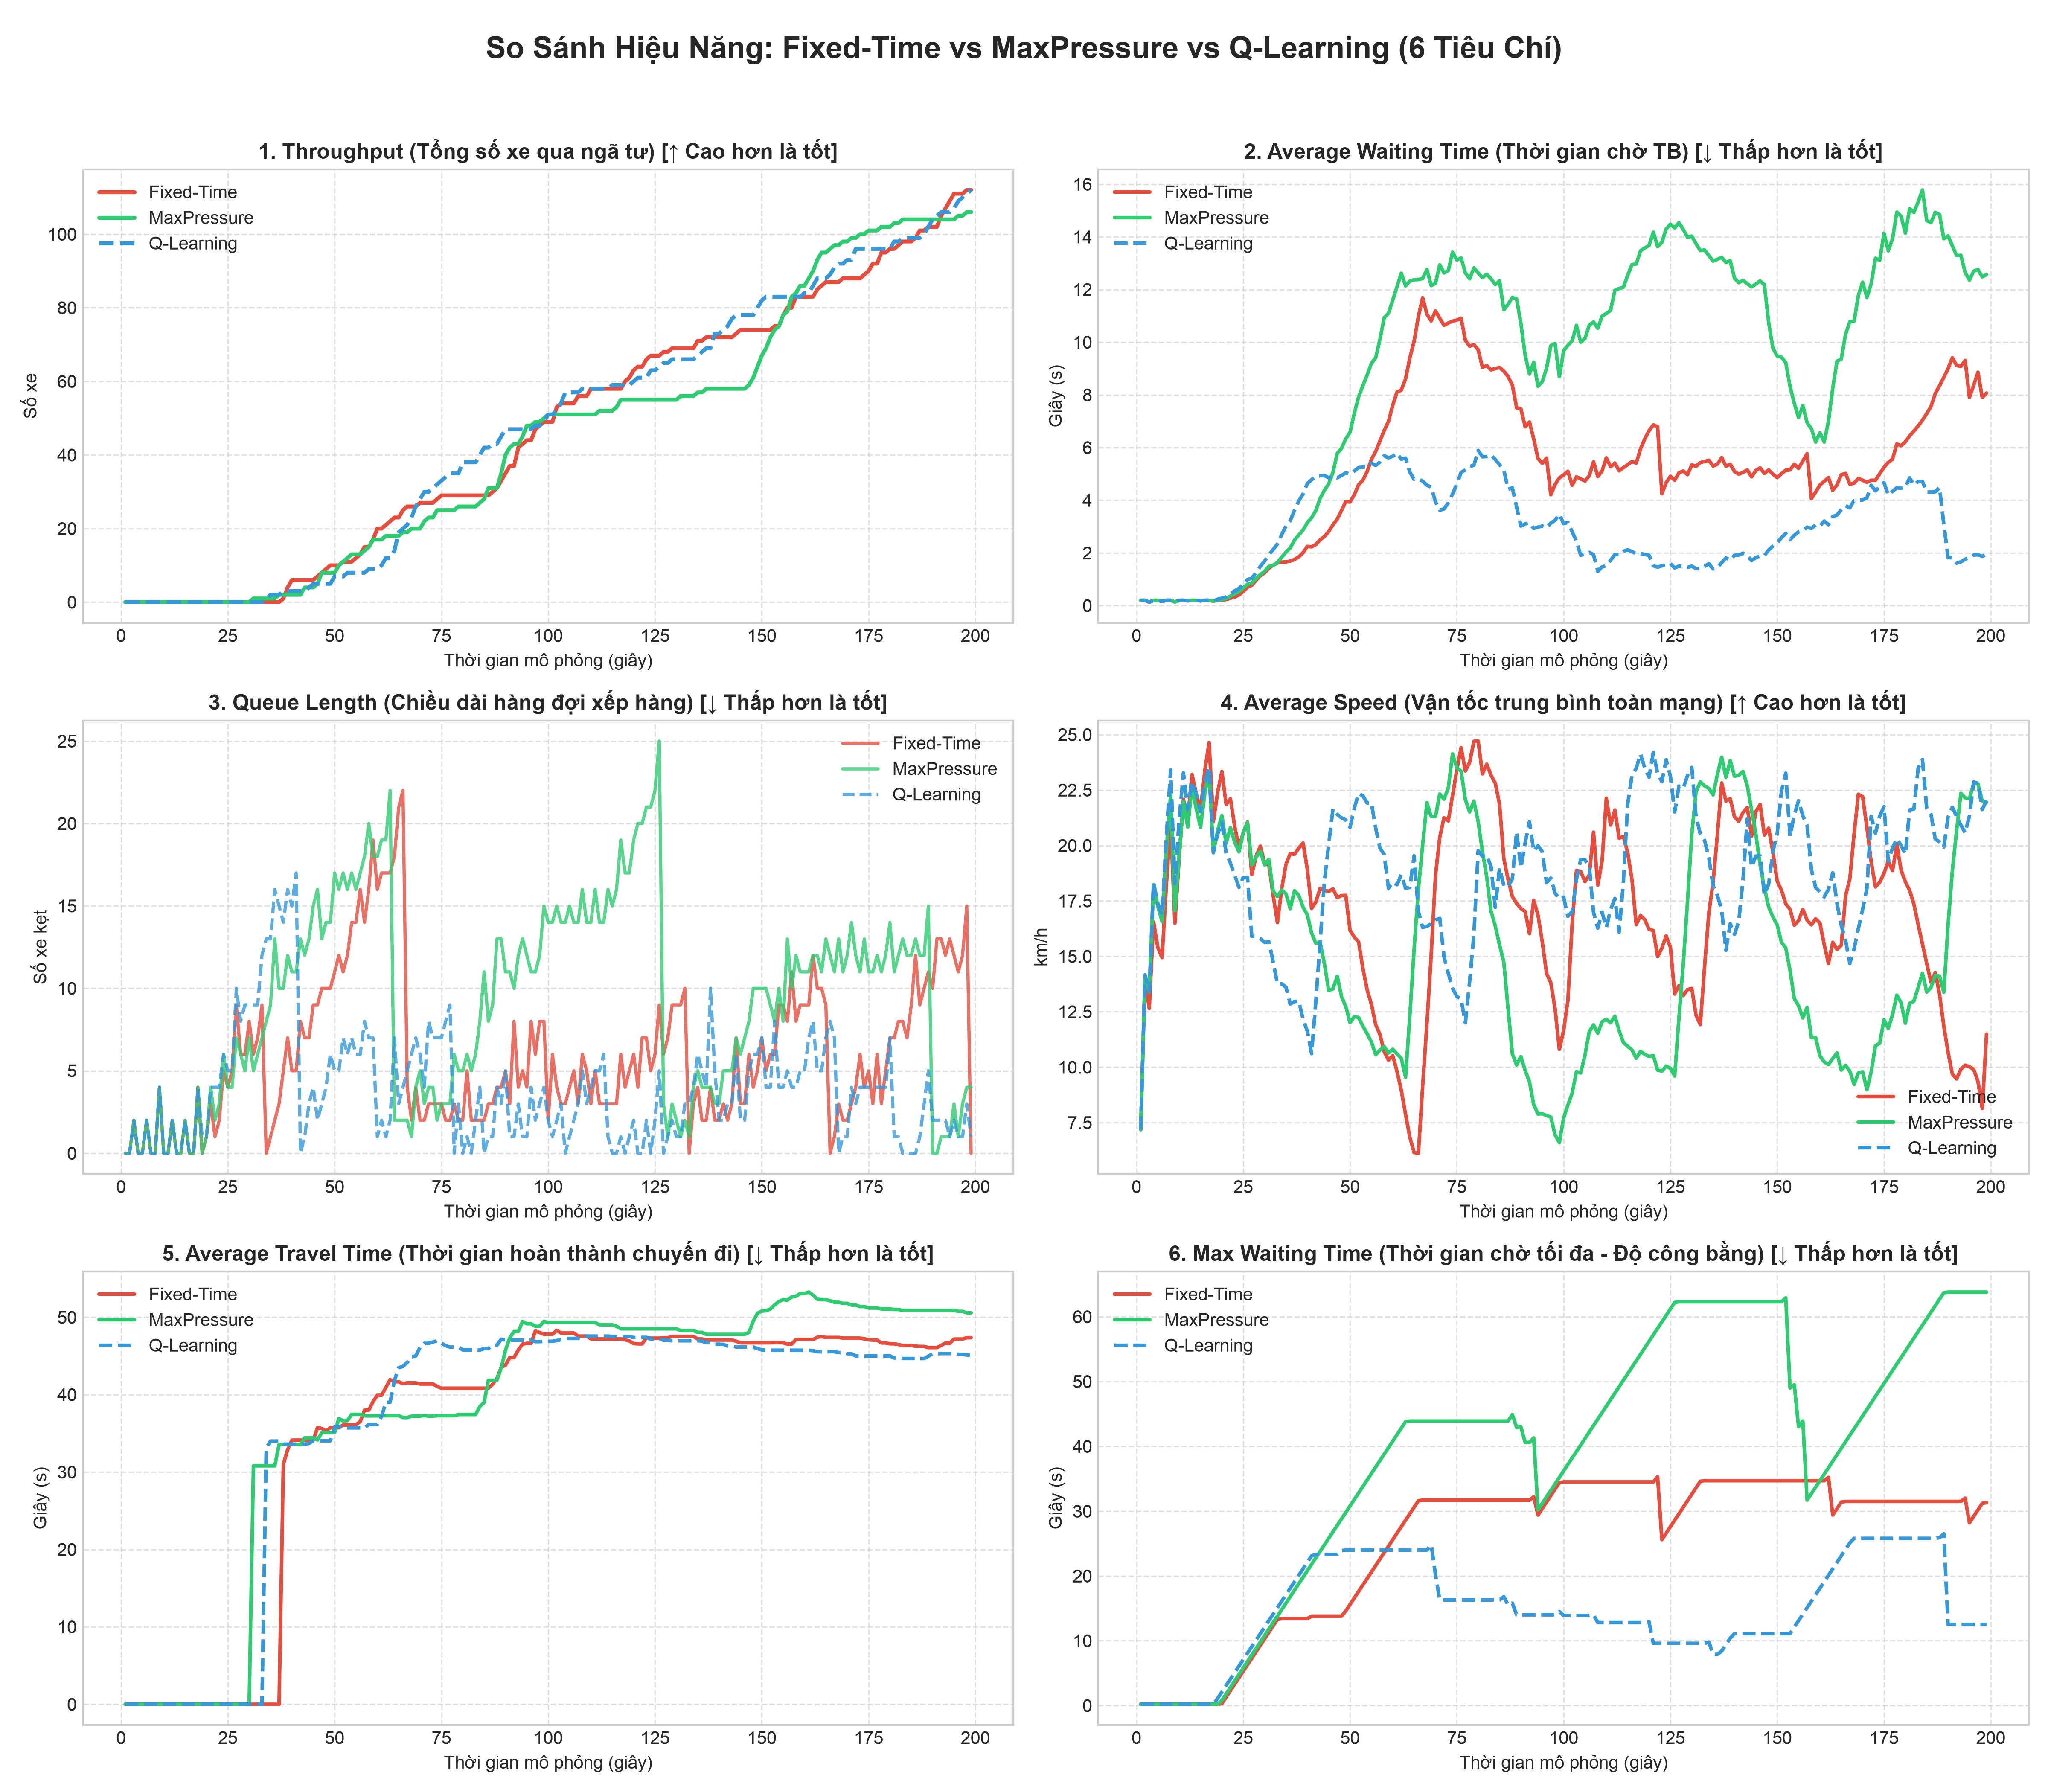
\includegraphics[width=1.15\textwidth]{comparison_results/traffic_comparison_3models_6metrics.png}}
\end{figure}

\end{document}